\documentclass{article}
\usepackage{amsmath}
\usepackage{tikz}
\begin{document}

\title{Electricity and Magnetism - Lecture 2 Notes}
\author{Joshua Clement}
\maketitle

\section*{Electric Field Strength}
\begin{itemize}
    \item \textbf{Electric Forces} are typically much stronger than \textbf{gravitational forces}.
    \item \textbf{Electric field} is a vector field that defines a vector at each point in space.
    \begin{itemize}
        \item Represented graphically with arrows or lines parallel to the field.
        \item Measured in \textbf{N/C}.
        \item Greater \textbf{line density} indicates a stronger electric field.
    \end{itemize}
\end{itemize}

\section*{Electric Field of Uniformly Charged Spherical Shell}
\begin{itemize}
    \item \textbf{Outside the Shell} (\(r > R\)):
    \[
    \vec{E} = \frac{1}{4\pi\epsilon_0} \frac{Q}{r^2} \hat{r}
    \]
    \item \textbf{Inside the Shell} (\(r < R\)):
    \[
    E = 0
    \]
    \item The electric field outside behaves like that of a \textbf{point charge}.
    \item Calculations involve the \textbf{superposition principle} and \textbf{Gauss' law}.
\end{itemize}

\section*{Superposition Principle}
\begin{itemize}
    \item The net electric field at any point is the \textbf{vector sum} of the individual fields from all charges.
    \item Electric field from a charged particle is \textbf{unaffected} by the presence of other charges.
\end{itemize}

\section*{Electric Dipole}


\begin{figure}[h!]
    \centering
    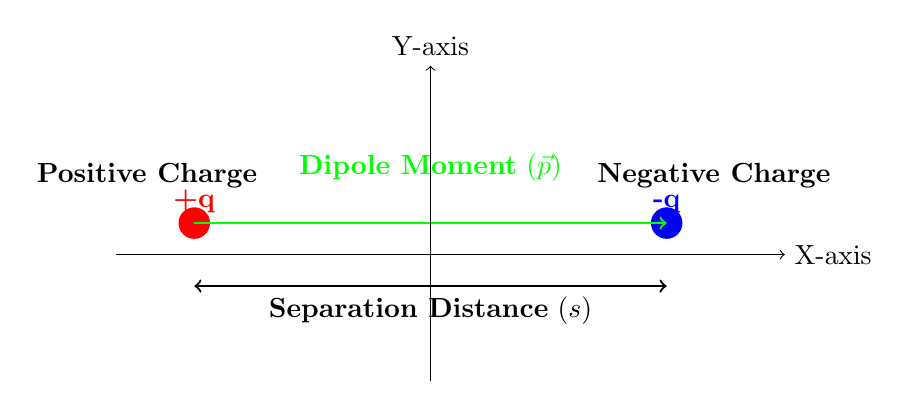
\begin{tikzpicture}
        % Draw positive charge (+q)
        \fill[red] (-3,0) circle (0.2) node[above] {\textbf{+q}};
        % Draw negative charge (-q)
        \fill[blue] (3,0) circle (0.2) node[above] {\textbf{-q}};

        % Draw the dipole moment vector
        \draw[->, thick, green] (-3, 0) -- (3, 0) node[midway, above, yshift=0.4cm, text=green] {\textbf{Dipole Moment} (\(\vec{p}\))};

        % Draw the distance between charges (s)
        \draw[<->, thick] (-3, -0.8) -- (3, -0.8) node[midway, below] {\textbf{Separation Distance} (\(s\))};

        % Labels for positive and negative charges
        \node at (-3.6,.6) {\textbf{Positive Charge}};
        \node at (3.6,.6) {\textbf{Negative Charge}};

        % Coordinate axes for better orientation
        \draw[->] (-4,-.4) -- (4.5,-.4) node[right] {X-axis};
        \draw[->] (0,-2) -- (0,2) node[above] {Y-axis};
    \end{tikzpicture}
    \caption{Graphical representation of an electric dipole showing positive (+q) and negative (-q) charges, dipole moment (\(\vec{p}\)), and separation distance (\(s\)).}
    \label{fig:dipole}
\end{figure}


\begin{itemize}
    \item \textbf{Electric Dipole}: Consists of two equal but opposite charges, \(+q\) and \(-q\), separated by distance \(s\).
    \item \textbf{Dipole Moment (\(\vec{p}\))}:
    \[
    \vec{p} = q \vec{s}
    \]
    \[
    or
    \]
    \[
    \vec{p} = qs\hat{s}
    \]
    \item Units: \textbf{C·m}.
    \item \textbf{Importance}:
    \begin{itemize}
        \item Neutral matter contains both positive and negative charges.
        \item \textbf{Far away}, the electric field of neutral matter approximates to that of a dipole.
        \item Dipoles are common in nature, e.g., \textbf{HCl molecule}.
    \end{itemize}
    \item \textbf{Electric Field of Dipole}:
    \[
        p = qs
    \]
    \begin{itemize}
        \item \textbf{Along the Axis} (\(r \gg s\)):
        \[
        \vec{E}_{\text{axis}} = \frac{1}{4\pi\epsilon_0} \frac{2p}{r^3} \hat{p}
        \]
        \item \textbf{Along Bisecting Plane}:
        \[
        \vec{E}_{\perp} = -\frac{1}{4\pi\epsilon_0} \frac{p}{r^3} \hat{p}
        \]
    \end{itemize}
\end{itemize}

\section*{Dipole in Uniform Electric Field}
\begin{itemize}
    \item A dipole in a \textbf{uniform electric field} experiences \textbf{torque}.
    \[
    \tau = \vec{p} \times \vec{E}_{\text{app}}
    \]
    \item \textbf{Equilibrium Position}: Minimizes potential energy.
    \[
    U = -\vec{p} \cdot \vec{E}_{\text{app}}
    \]
\end{itemize}

\end{document}